\chapter{ADS-B signals}\label{ch:adsbsig}

Automatic dependent surveillance-broadcast (ADS-B) is a system in which aircraft continually transmit their identity and GPS-derived navigational information. ADS-B networks for air traffic monitoring have already been implemented in areas around the world, but ground stations cannot be installed in mid-ocean and are difficult to maintain in the Arctic, leaving a coverage gap for oceanic and high latitude airspace \citep{FlyingLab}. Therefore a solution can be to monitor the signals with a low orbit satellite using an antenna matched to the frequencies of the ADS-B.There are currently three types of ADS-B transmissions, including the 1090 MHz extended squitter (ES), the 978 MHz universal access transceiver (UAT), and the VHF data link (VDL) mode 4 operating between 108 and 137 MHz.
 \\
An ADS-B message is 112 bits long and the transmission takes 120us. The mudulation is pulsed RF and the package consist of 5 parts. The first part is Downlink Format which tells that this is an ADS-B signal, second part is Additional Identifier which has different meaning within each ADS-B subtype. The third is the ICAO which is the unique identifier of the aircraft. The fourth is the DATA which contains several informations including aircraft operation status, airborne position and velocities measured from different sensors. The fifth and last is the checksum \citep{Modesorg}. It is observed that the ADS-B signal is a unencrypted signal which makes it easy to detect and therefore also vulnerable to attacks \citep{Attacks}.       

\begin{figure}[h]
\centering 
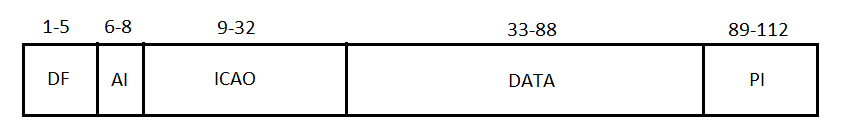
\includegraphics[scale = 0.5]{figures/adsb_signals/adsb_message.png}
\caption{112 bit long ADS-B message}
\label{fig:adsb_mes}
\end{figure}


\textbf{1090MHz Mode S Extended Squitter}\\
This is the most common frequency in ADS-B. It uses a single channel at 1090MHz and is used for communication from aircraft to ground only. The message is sent in intervals determined by the aircraft commonly every second.   
\\
\textbf{978MHz Universal Acces Transceiver}\\
This is a newer standard that communicates from aircraft to aircraft. It uses a single frequency at 978MHz.  
\\
\textbf{108-137MHz VHF Data Link Mode 4}\\
This is most commonly used at small airplanes. It is multi-channel where the frequency depends upon the local regulations. The channel spacing is 1MHz. 